\documentclass[a4paper,oneside]{article}
\usepackage[a4paper, margin=2cm, lmargin=2.5cm, rmargin=2.5cm, bmargin=1.2cm]{geometry}
\headsep=5pt
\usepackage{amsmath}
\usepackage{amsthm}
\usepackage{amsfonts}
\usepackage{xeCJK}       %讓中英文字體分開設置

\setCJKmainfont{Noto Sans CJK TC}
\XeTeXlinebreaklocale "zh"             %這兩行一定要加,中文才能自動換行
\XeTeXlinebreakskip = 0pt plus 1pt

\usepackage{enumitem}
\usepackage{algpseudocode}
\usepackage{tikz}
% Tikz settings optimized for causal graphs.
% Just copy-paste this part
\usetikzlibrary{shapes,decorations,arrows,calc,arrows.meta,fit,positioning}
\tikzset{
    -Latex,auto,node distance =1 cm and 1 cm,semithick,
    state/.style ={ellipse, draw, minimum width = 0.7 cm},
    point/.style = {circle, draw, inner sep=0.04cm,fill,node contents={}},
    bidirected/.style={Latex-Latex,dashed},
    el/.style = {inner sep=2pt, align=left, sloped}
}
\usepackage{listings}
\usepackage[T1]{fontenc}
\usepackage{fancyhdr}
\usepackage{url}
\usepackage{color}
\usepackage{graphicx}
\usepackage{tgcursor}
\usepackage[compact]{titlesec}
\titlespacing{\section}{0pt}{*0}{*0}
\titlespacing{\subsection}{0pt}{*0}{*0}
\titleformat{\section}[hang]
  {\normalfont\bfseries}
  {}
  {0em}
  {\Large \thesection\hspace{0.6em}}
\titleformat{\subsection}[hang]
  {\normalfont\bfseries}
  {}
  {0em}
  {\large \thesubsection\hspace{0.6em}}

\pagestyle{fancy}
\fancyfoot{}
\fancyhead[L]{Introduction to Embedded Systems Design and Implementation}
\fancyhead[R]{Page \thepage}
\definecolor{deeper}{gray}{.8}

\renewcommand*{\ttdefault}{pcr}
\lstset{
		basicstyle=\footnotesize\ttfamily,
		tabsize=2,
		breaklines=true,
}
\setlist{leftmargin=\parindent}

\setlength{\parindent}{1em}
\graphicspath{ {./images/} }
\titlespacing{\section}{0pc}{1pc}{0.5pc}
\titlespacing{\subsection}{0pc}{1pc}{0.5pc}
\titlespacing{\subsubsection}{0pc}{1pc}{0.5pc}
\linespread{1.2}

\begin{document}
\title{2020/03/20 Discussion}
\author{0616014 楊政道}
\maketitle
\thispagestyle{fancy}
\section{Discussion 1}
\subsection{Why do we need to put resistors in the circuit?}
\begin{figure}[!h]
\begin{center} 
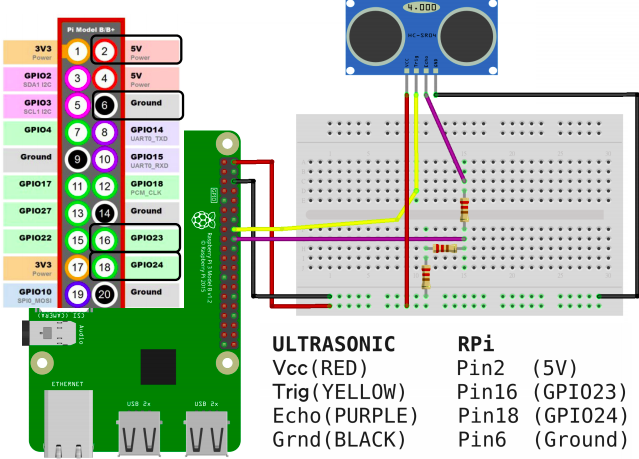
\includegraphics[width=8cm]{resistor.png} 
\caption{resistor layout}
\end{center} 
\end{figure} 
\paragraph{}
Because the output voltage from the \texttt{HC-SR04} Ultrasonic module is \texttt{5V} but the maximum limitation of the voltage to the pin on the raspberrypi is \texttt{3.3V}, we need to reduce the voltage by 3 same resistors to make the voltage into \texttt{5 * 2 / 3 = 3.3V}.
\subsection{Read datasheet. What is the max and min distance that it can detect?}
\begin{figure}[!h]
\begin{center} 
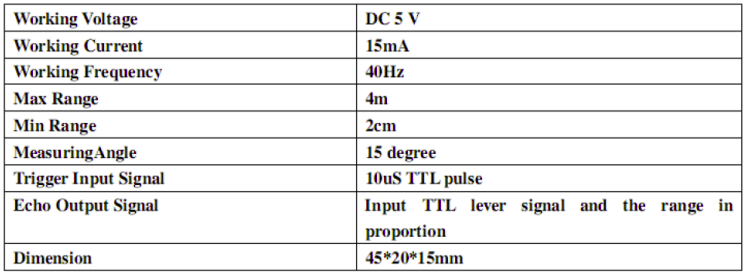
\includegraphics[width=10cm]{HC-SR04-datasheet.png} 
\caption{HC-SR04 datasheet}
\end{center} 
\end{figure} 
\paragraph{}
According to the datasheet of the HC-SR04 module, the maximum range it can detect is 4 meters and the minimun range it can detect is 2 centimeter.
\subsection{Based on distance measurement, is there any other application?}
\begin{figure}[!h]
\begin{center} 
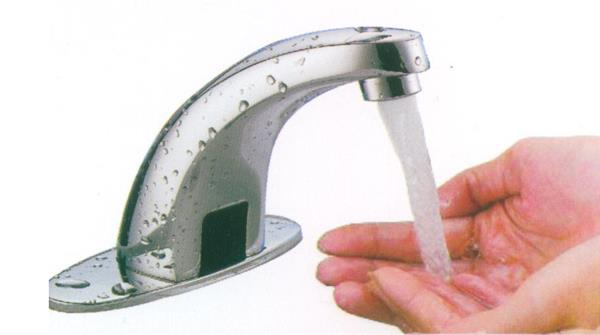
\includegraphics[width=8cm]{faucet.jpeg} 
\caption{induction faucat}
\end{center} 
\end{figure} 
\paragraph{}
One of the applications based on distance measurement is induction faucats. The distance sensor can detect hands are coming and turn the faucet on.
\begin{figure}[!h]
\begin{center} 
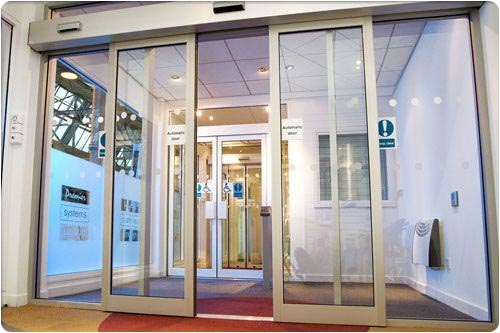
\includegraphics[width=8cm]{automatic-door.jpg} 
\caption{automatic door}
\end{center} 
\end{figure} 
\paragraph{}
Another one of the applications based on distance measurement is automatic door. When someone is close to the door, the door will open.
\subsection{If we want to use Physical PIN number, how to modify the code?}
\section{Discussion 2}
\begin{figure}[!h]
\begin{center} 
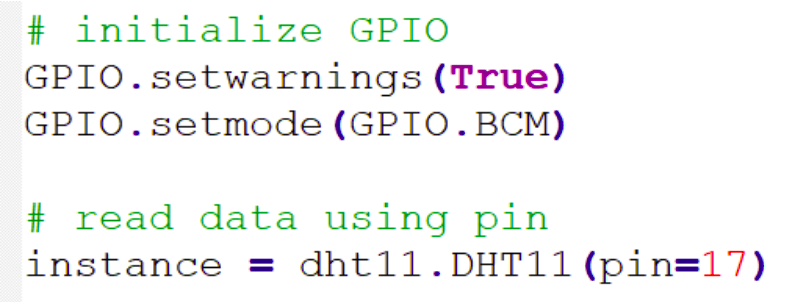
\includegraphics[width=8cm]{sample.png} 
\caption{sample code}
\end{center} 
\end{figure} 
\paragraph{}
We can use \texttt{GPIO.setmode(GPIO.BOARD)} so that we can use physical pin numbers of the raspberry pi.

\end{document}
